\section{Polymorphism}
\label{sec:polymorphyism}

Polymorphism is the ability of an entity to show diferent shapes or
forms. In biology, polymorphic animals can exist isa variety of
different forms, e.g.~male and female animals, or different blood
types. In materials science, polymorphic material can exist in a
variety of different crystaline configurations (e.g.~calcite and
aragonite). 

In computer science, polymorphism appears at many levels. In
Programming in Java, we interested in two types of polymorphism:
polymorphic classes and polymorphic methods. The former is usually
referred to as \emph{generic types}, while the latter is usually
called \emph{method overloading}. 

\section{Generic types/classes}
\label{sec:generic-types}

A generic type or generic class
is a complex type that can be combined with many other
different types. The most common application of generic types is for
``container'' classes like lists, stacks, and queues. 

When we were creating our own dynamic classes in previous weeks, they
were usually attached to a type: lists of strings, stacks of integers,
etc. A generic class, on the other hand, could work the same for many
types, saving programmers from the hassle of having different but very
similar types (e.g. stacks) for each different type of data they want
to use (i.e.~string stacks, integer stacks, patient stacks, etc). 

\subsection{Using generic classes}
\label{sec:using-gener-class}

A generic class is very similar to a normal class. The only
difference ---and it is a crucial one--- is that it uses one or more
type variable to specify the types used in its code. Type variables
are specified in low quotes (``$<$'', ``$>$''). Let's see an
example of a generic interface, a stack (comments are removed for
brevity): 

\begin{verbatim}
    public interface Stack<T> {
        void push(T object);
        T pop();
    }
\end{verbatim}

If we wanted to implement this interface using arrays, it could look
like this (comments removed for brevity): 

\begin{verbatim}
    public class ArrayStack<T> {
        private T[] contents;
        private int headIndex; 

        public T pop() {
            if (headIndex == 0) {
                return null;
            }
            headIndex--;
            T result = contents[headIndex];
            contents[headIndex] = null;
            return result;
        }
        // ... constructor and other methods would be here ...
    }
\end{verbatim}

As you can see, there are two main differences between a normal class
and a generic class (and their methods): 

\begin{itemize}
\item The name of the class is extended to include the type, by using
  a variable type in low quotes. Capital T (for ``type'') is a common
  name for variable types, and by convention variable types are
  usually capital single letters, but any valid identifier can be
  used.
\item The variable type can be used in every place where a type
  (simple or complex) should be: parameter types, return types, and
  for declaring new variables. 
\end{itemize}

How are generic interface and classes used? Look at this code:

\begin{verbatim}
    // ...
    Stack<Integer> myNumberStack = new ArrayStack<Integer>();
    Stack<String> myStringStack = new ArrayStack<String>();
    myNumberStack.push(1);
    myStringStack.push("Test string!");
    // ...
\end{verbatim}

As you can see, the same interface and class can be used to handle
different types, i.e.~Integers and Strings in this case. Generic types
must be based on complex types (classes), not simple types. Boxed
types are useful if you need a generic type based on one of the
primitives. This is why the example uses a \verb+Stack<Integer>+; if you try
to create a \verb+Stack<int>+, the compiler will complain. 

\subsection{Restricting generic types}
\label{sec:restr-gener-types}

There are situations in which you want to create a generic type based
on some types, but not every single type out there. For example, you
may want to use in your program a list of \verb+Person+, but you do
not want lists of string or hospital appearing in your code from other
modules. 

Restricting the type is easy and can be done in more than one way. For
now, we will look at just one way of doing it by means of
interfaces. Look at this example:

\begin{verbatim}
    public interface List<P implements Person> {
        void push(P object);
        P pop();
    }
\end{verbatim}

In this case, we are using P instead of T for the type variable to
make it clearer that it must be a Person, not just any type. The
compiler knows that any type that we combine this list with must be a
class that extends the interface \verb+Person+. Therefore, we will be
able to create a \verb+List<KidPerson>+ but not a
\verb+List<Integer>+. If we try to do the latter, the compiler will
complain. 

\subsection{Conclusion}
\label{sec:conclusion-2}

Benefits of generic classes: 

\begin{itemize}
\item compilation detects errors
\item less repetition of code
\end{itemize}

Drawbacks

\begin{itemize}
\item Code very verbose
\item If they are abused, they make the code unreadable
\end{itemize}

\section{Method overloading}
\label{sec:method-overloading}

...

\section{Introduction to upcasting}
\label{sec:upcasting}

There is a third type of
polymorphism in Java that is simpler but very important. We have
already seen how it works, although we have not used its proper name
until now.
%We are already familiar with \emph{upcasting}, although we have not
%called it like that. 
We have been using it every time we have declared
a variable by using an interface: 

\begin{verbatim}
    List patientList;
    patientList = new ArrayPatientList();
\end{verbatim}

We know that it is good practice to work with interface names for our
data types, rather than to use the class names directly. The interface
allows the programmer to abstract from all the implementation details
of the class and work with just its public behaviour, i.e.~the methods
defined on the interface. This is upcasting, and it is similar to the
casting of simple types we have already seen; you just need to know
that, by convention, interfaces are imagined to be ``up'' and specific
classes are imagined to be ``down'', so casting from class to
interface is up-casting. (The origin in computer science is almost
always up: the root of a tree, the interface of a class, etc). 

\begin{figure}[hbtp]
  \centering
  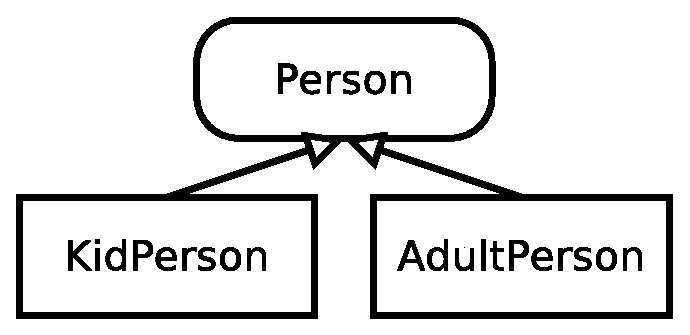
\includegraphics[height=3cm]{gfx/class_diagram-person}
  \caption{Interface Person is implemented by classes KidPerson and
    AdultPerson. By convention, the interface is represented ``up'' and
    the classes are represented ``down''.} 
  \label{fig:updown}
\end{figure}

We will see more about upcasting (and downcasting) in the following
sections. 



%%% Local Variables:
%%% mode: latex
%%% TeX-master: "main"
%%% End:
